% !TEX root = ../Main.tex

\chapter[Methods for Simulating Stabilizer Circuits]{Methods for Simulating Stabilizer\\ Circuits}
\label{chap:stabilizers}

\section{Introduction}\label{sec:stabilizer-intro}
% Stabilizer circuits are an intersting class of circuits
% Capture many seemingly quantum features
% Recap definition
% Some of this is probably meant for intro instead
In the previous chapter (INSERT REFERENCE), we briefly introduced the notion of stabilizer circuits as a class of efficiently simulable quantum computations. In this chapter, we revisit stabilizer circuits in detail, with a focus on different classical data structures for encoding stabilizer states and the corresponding algorithms for simulations.\par
Several informal definitions of stabilizer circuits have been used in the quantum computing literature~\cite{Gottesman1998b,Aaronson2004,VandenNest2008,Seddon2019}. However, what each definition has in common is that the operations $\mathcal{E}$ acting on an abelian subgroup $\mathcal{S} \subseteq \mathcal{P}_{n}$ generate a new subgroup $\mathcal{S'}\subseteq \mathcal{P}_{n}$. These groups $\mathcal{S}$ are also called a stabilizer groups.\par
In this thesis, we focus exclusively on stabilizer circuits acting on pure states $\ket{\phi}$ called stabilizer states. These can be entirely characterized by their associated stabilizer group as
\begin{equation}
    s\ket{\phi}=\ket{\phi}\;\forall s\in\mathcal{S}
\end{equation}
For an $n$-qubit state, the group $\mathcal{S}$ has $2^{n}$ elements~\cite{Gottesman1998b}. As $\mathcal{S}$ is also abelian, this means it can be described by a generating set with $n$ elements,
\begin{equation}
    \mathcal{S} = \langle g_{1}, g_{2},\dots,g_{n}\rangle \; : g_{i}\in\mathcal{S},
\end{equation}
which are commonly referred to as the `stabilizers' of the state $\ket{\phi}$. We also note that this definition allows us to write
\begin{equation}
    \ketbra{\phi} = \frac{1}{2^{n}}\sum_{s\in\mathcal{S}} s = \frac{1}{2^{n}}\prod_{i=1}^{n}\left(\mathbb{I}+g_{i}\right)
\end{equation}
Given that these circuits map stabilizer states to other stabilizer states, this means they must be built up of unitary operations $U$ which map Pauli operators to other Pauli operators under conjugation. This set is commonly denoted as $\mathcal{C}_{2}$, or the `second level of the Clifford hierarchy' 
\begin{align}
    \mathcal{C}_{2} &\equiv \{U\,:\,UPU^{\dagger}\in\mathcal{P}_{n}\;\forall P\in\mathcal{P}_{n}\} \label{eq:c2}\\
    \mathcal{C}_{j} &\equiv \{U\,:\,UPU^{\dagger}\in\mathcal{C}_{j-1}\;\forall P\in\mathcal{P}_{n}\} \label{eq:cj}
\end{align}
where in Eq.~\ref{eq:cj} we have also introduced the (recursive) definition for level $j$ of the Clifford hierarchy. From this definition
\begin{equation}
    V\mathcal{S}V^{\dagger}=\langle Vg_{i}V^{\dagger}\rangle = \langle g_{i}' \rangle = \mathcal{S}'
\end{equation}
%TODO: Do we need to explain measurement or just cite it? Maybe this comes up later in the implementation...
We also allow stabilizer circuits to contain measurements in the Pauli basis~\cite{Gottesman1998b}.
\subsubsection*{Simulating stabilizer circuits}
% Classical simulabiltiy follows from gate updates and encoding
% Introduce tableaux, and classical encoding
From the above definitions, we can see that simulating a stabilizer circuit on $n$ qubits corresponds to updating the $n$ stabilizer generators for each unitary and measurement we apply. As the number of generators grows linearly in the number of qubits, if these group updates can be computed in time $O\left(\poly (n)\right)$ then it follows the circuits can be efficiently simulated clasically.\par
The first proof of this was given by Gottesman in \cite{Gottesman1998b}, by showing through examples that stabilizer updates can be quickly computed for the CNOT, H and S gates, and for single qubit Pauli measurements. This is significant as the $n$ qubit Clifford group can be entirely generated from these gates.
\begin{equation}
    \mathcal{C}_{2} = \langle CNOT_{i,j},\, H_{i},\, S_{i}\,:i,j\in \mathbb{Z}_{n}\rangle. \label{eq:cliffordgen}
\end{equation}
This result is typically referred to as the `Gottesman-Knill' theorem.\par
A more formal proof follows from the work of Dehaene \& de-Moor, who showed that the action of Clifford unitaries on Pauli operators corresponds to multiplication of $(2n+1)\times (2n+1)$ symplectic binary matrices with $(2n+1)$-bit binary vectors~\cite{Dehaene2003}. The dimension of these elements also grows just linearly in the number of qubits, and as matrix multiplication requires time $O(n^{2.37})$ it follows that we can update the stabilizers in $O(mn^{2.73})$ for $m$ Clifford gates.\par
This work was then extended by Aaronson \& Gottesman, who introduced an efficient data structure for stabilizer groups, and algorithms for their updates under Clifford gates and Pauli measurement~\cite{Aaronson2004}. This method avoids the need for matrix multiplications, instead providing direct update rules allowing stabilizer circuits to be simulated in $O(n^{2})$.\par
Since 2004, there have been several papers looking at different data structures and algorithms for simulating stabilizer circuits of the type we consider here. For example, a method based on encoding stabilizer states as graphs~\cite{Anders2006}, refinements of the Aaronson \& Gottesman encoding~\cite{Garcia2012}, and an encoding using affine spaces and phase polynomials~\cite{VandenNest2008,Bravyi2016}.\par
In the rest of this section, we will discuss different aspects of simulating stabilizer circuits, focusing on updating stabilizer states under gates and measurements, computing stabilizer inner products, and the connections between stabilizer circuits and states.
% \clearpage
\subsection{Tableau Encodings of Stabilizer States}\label{sec:sympencoding}
The method in \cite{Aaronson2004} is based on a classical data structure they call the `stabilizer tableau', a collection of Pauli matrices that define the stabilizer group, encoded using the binary symplectic representation of \cite{Dehaene2003}
\begin{equation} P = i^{\delta}-1^{\epsilon} \bigotimes_{i=1}^{n} x_{i}z_{i}\end{equation}
where the Pauli matrix at qubit $i$ is defined by two binary bits such that
\begin{equation}
    x_{i}z_{i} = \begin{cases}
    I & x_{i}=z_{i}=0\\
    X & x_{i}=1, z_{i}=0 \\ 
    Z  &x_{i}=0, z_{i}=1 \\
    Y  &x_{i}=z_{i}=1
    \end{cases}
\end{equation}
Together with the $\delta$ and $\epsilon$ phases, a generic Pauli operator can be encoded in $2n+2$ bits; two bits to encode the phase, and two $n$-bit binary strings $\tilde{x},\tilde{z}\in\mathbb{Z}_{2}^{n}$ to encode the Pauli acting on each qubit, commonly referred to as `x-bits' and `z-bits' respectively. In this picture, multiplication of Pauli operators corresponds to addition of $x$ and $z$ bits modulo 2, with some additional, efficiently computable function for correcting the phase~\cite{Dehaene2003}
\begin{align}
    P Q &= i^{\delta_{pq}}-1^{\epsilon_{pq}}\bigotimes_{i=1}^{n}x_{i}' z_{i}' \\
    x'_{i} &= x_{pi}\oplus x_{qi} \\
    z'_{i} &= z_{pi} \oplus x_{qi}
\end{align}
where $\delta_{pq} = \delta_{p}\oplus \delta_{q}$, $\epsilon_{qr} = f(\tilde{x}_{p}, \tilde{z}_{p}, \tilde{x}_{q}, \tilde{z}_{q})$.\par
%%Tableau definition, drops an extra factor of n bits
%% Gate updates
In stabilizer groups, we can restrict ourselves to considering Pauli operators with only real phase. This is because if $iP\in\mathcal{S}$, then $(iP)^{2}=-I\in\mathcal{S}$. But, this implies that $-I\ket{\phi}=\ket{\phi}$, which is a contradiction.\par
While only $n$ generators $S_{i}$ are needed to characterize the stabilizer group $\mathcal{S}$, the tableau also includes an additional $2n$ operators called `destabilizers' $D_{i}\in\mathcal{P}_{n}$. Together, these $2n$ operators generate all $4^{n}$ elements of $\mathcal{P}_{n}$.\par
There are many possible choices of destabilizer, but the tableau chooses operators such that~\cite{Aaronson2004}
\begin{align*}
    \comm{D_{i}}{D_{j}} &= 0\;\forall\, i, j \,\in \{1,\dots,n\} \\
    \comm{D_{i}}{S_{j}} &= 0 \iff i\neq j \\
    \acomm{D_{i}}{S_{i}} &= 0 
\end{align*}
Altogether, the full tableau has spatial complexity $4n^{2}+2n$. These are sometimes referred to as `Aaronson-Gottesman 'tableaux or `CHP' tableaux, after the software implementation by Aaronson~\cite{Aaronson2004b}.
\begin{figure}[H]
\begin{equation}
\kbordermatrix{~ & ~ & ~ & ~ & ~ & ~ & ~ & ~ & ~ & ~\\
    \mathcal{D}_{1} & x_{1,1} & \cdots & x_{1,n} & \omit\vrule & z_{1,n} & \cdots & z_{1,n} & \omit\vrule & r_{1} \\
    \vdots & \vdots & \ddots & \vdots &\omit\vrule & \vdots & \ddots & \vdots & \omit\vrule  &\vdots \\
    \mathcal{D}_{n} & x_{n,1} & \cdots & x_{n,n} & \omit\vrule & z_{n,1} & \cdots & z_{n,n} & \omit\vrule & r_{n}\\ \hline
    \mathcal{S}_{1} & x_{n+1,n} & \cdots & x_{n+1,n} & \omit\vrule & z_{n+1,1} & \cdots & z_{n+1,n} & \omit\vrule & r_{n+1}\\
    \vdots & \vdots & \ddots & \vdots & \omit\vrule & \vdots & \ddots & \vdots & \omit\vrule & \vdots \\
    \mathcal{S}_{n} & x_{2n, 1} & \cdots & x_{2n, n} & \omit\vrule & z_{2n,1} & \cdots & z_{2n,n}&\omit\vrule&r_{2n}
    }
\end{equation}
\caption{Example of a `CHP' tableau, where the first $n$ rows are the Destabilizers and the next $n$ rows are the stabilizers. The $2n+1$th column gives that phase $-1^{r_{i}}$ for each operator.}
\label{fig:ExampleCHP}
\end{figure}
\subsubsection*{Simulating Gates}
Gate updates for each individual operator in the tableau can be computed constant time. For example, the Hadamard transforms single qubit Pauli matrices under conjugation as
\begin{equation}
    HPH^{\dagger} = \begin{cases}
        I & P=I\\
        Z & P=X\\
        X & P=Z\\
        -Y & P=Y
        \end{cases}
\end{equation}
In the symplectic form, we then have to update the $i$th Pauli operator as
\begin{equation}
    x_{i}'z_{i}' = (x_{i}\oplus p)(z_{i}\oplus p) \; : \; p = x_{i} \oplus z_{i}
\end{equation}
and the phase as
\begin{equation}
\delta' = \delta \oplus \left(x_{i}\wedge z_{i}\right)
\end{equation}
Similar update rules exist for the CNOT and S gates, which together generate the $n$ qubit Clifford group. As there are $O(n)$ operators in the tableau, and each update is constant time, gate updates overall take $O\left(2n\right)$~\cite{Aaronson2004}. This is in contrast to the $O(n^{2.37})$ complexity of~\cite{Dehaene2003}
\subsubsection*{Simulating Measurements}
The addition of the destabilizer information is  used to speed up the simulation of Pauli measurements on Stabilizer states. Measuring some operator $P$ on a stabilizer state will always produce either a deterministic outcome, or an equiprobable random outcome~\cite{Gottesman1998b}.\par
If the outcome is deterministic, then $\pm P$ is in the stabilizer group, and the outcome is $+1$ or $-1$ respectively. Using the stabilizer genereators, this allows us to write 
\begin{equation}
    \comm{P}{S_{i}}=0\;\forall S_{i}\in\mathcal{S} \implies \prod_{i}c_{i}S_{i} = \pm P. \label{eq:det_requirement}
\end{equation}
for binary coefficients $c_{i}$.\par
Checking if the outcome is deterministic takes $O(n^{2})$ time in general, using the symplectic inner product to check the commutation relations~\cite{Dehaene2003}. However, checking which measurement outcome occurs involves computing the coefficients $c_{i}$. In the symplectic form, thiscan be rewritten as
\[
    Ac=P
\]
where $c$ is a binary vector, $A$ is a matrix with each stabilizer as a column vector, $P$ is the operator to measure, and we have dropped the phase. Solving this would require inverting the matrix $A$, and take time $O(n^{3})$.\par
Aaronson \& Gottesman show that for single qubit mesurements, including destabilizer information instead allows us to compute the $c_{i}$ and the resulting measurement outcome in $O(n^{2})$. As this is a single qubit measurement, they also show that the commutivity relation requries checking only individual bits of the stabilizer vectors, also reducing that step to $O(n)$ time.\par
For random measurements, from Eq.~\ref{eq:det_requirement}, $\exists S_{i}:\acomm{S_{i}}{P}=0$, and it suffices to replace this stabilizer with $P$, and update the other elements of the group as $S_{j}'=PS_{j}$ iff $\acomm{S_{j}}{P}=0$~\cite{Gottesman1998b,Aaronson2004}.
\subsubsection*{`Canonical' Tableaux}
% A&G fix tableaux through initial state
There are multiple possible choices of generators for each stabilizer group/state. For example, for the Bell state $\ket{\phi^{+}}=\frac{1}{2}\left(\ket{00}+\ket{11}\right)$
\begin{align}
    \mathcal{S} = \{II, XX, -YY, ZZ\} = \langle XX,-YY\rangle = \langle XX, ZZ\rangle = \langle -YY,ZZ\rangle.
\end{align}
In simulation, tableau are fixed by choice of a convention. For example, it is possible to arrive at a `canonical' set of stabilizer generators using an algorithm which strongly resembles Gaussian elimination~\cite{Garcia2012}. This method rearranges the stabilizer rows of the tableau by multiplying and swapping generators, such that the overall stabilizer group is left unchanged. Computing this canonical form requires  time $O(n^{3})$~\cite{Garcia2012}.
\begin{figure}[H]
    \centering
    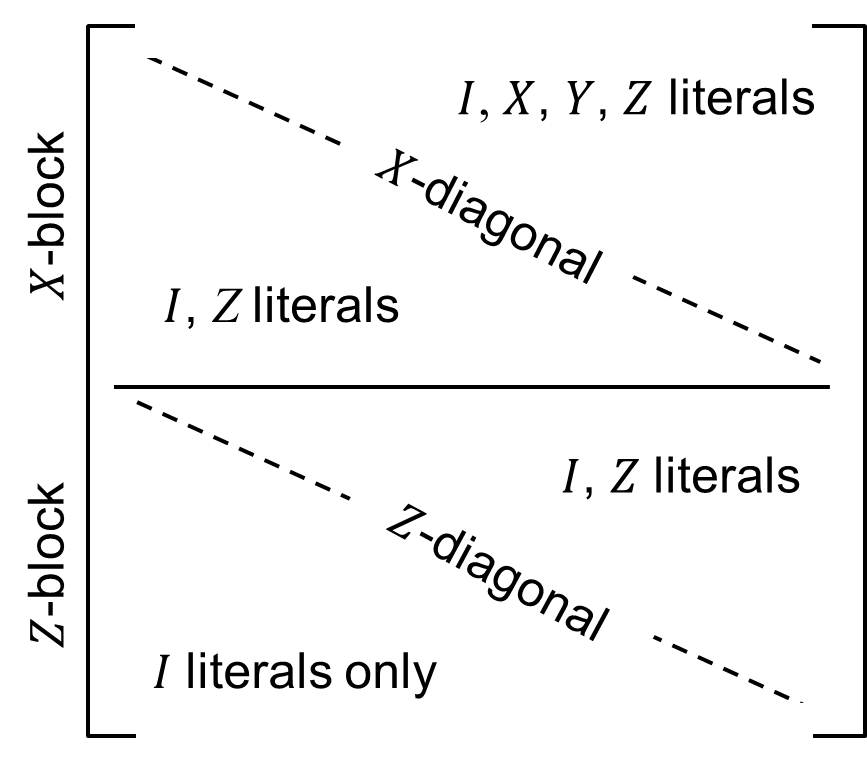
\includegraphics[width=0.45\linewidth]{stbmtx_inv.jpg}
    \caption{Representation of the canonical or `row-reduced' set of stabilizer generators. Figure taken from~\cite{Garcia2012}.}
\label{fig:canoncialtableau}
\end{figure}
These tableau can then be updated using the same methods as in \cite{Aaronson2004}, though this will in general not preserve the canonical form. Each Clifford gate will change one or two columns of the tableau, and thus an additional $O(n)$ row multiplications are required to restore it to canonical form, taking total time $O(n^{2})$ per gate~\cite{Garcia2015}.
Importantly this canonical tableau can also be used to compute deterministic measurement outcomes in time $O(n)$, and so this method can simulate measurement outcomes more efficiently at the cost of more expensive gate updates~\cite{Garcia2015}.\par
In contrast, Aaronson \& Gottesman fix the stabilizer tableau through an initial state, $\ket{0}^{\otimes n}$. The full tableau for this state looks like the identity matrix, with an additional zero-column for the phases. The tableau of a given state $\ket{\phi}$ is then built-up gate by gate using a stabilizer circuit $V:\ket{\phi}=V\ket{0^{\otimes n}}.$
\subsection{Connecting Stabilizer States and Circuits}
% Connection between clifford circuits and states
The convetion for `CHP' stabilizer tableaux mentioned above, and the definition of stabilizer circuits given in Section~\ref{sec:stabilizer-intro}, show that stabilizer states can also be defined by a stabilizer circuit and an initial state.\par
In \cite{Aaronson2004}, the authors derive examples of these `canonical circuits', and show that its possible for any stabilizer state to be synthesised by a unique circuit acting on the $\ket{0^{\otimes n}}$ state
\begin{equation}
    \ket{\phi} = V\ket{0} = H\;C\;S\;C\;S\;C \;H \; S \;C \;S \ket{0^{\otimes n}}\label{eq:chpcirc}
\end{equation}
where each letter denotes a layer made up of only Hadamard (H), CNOT (C) or S gates. The proof is based on  a sequence of operations reducing an arbitrary tableau to the identity matrix, each step of which corresponds to applying layers of a given Clifford gate~\cite{Aaronson2004}. As a corollary, the total number of gates in the canonical circuit for an $n$-qubit stabilizer state scales as $O(n\log (n))$~\cite{Aaronson2004}, based on previous work on synthesising $CNOT$ circuits with the $O(n\log (n))$ gates~\cite{Patel2003}, and that each $H$ and $P$ layer can act on at most $n$-qubits.\par
A slightly simpler canonical form was derived in 2008, which allows a stabilizer circuit to be written as
\begin{equation}
    \ket{\phi} = S\;CZ\;X\;C\;H \ket{0^{\otimes n}} \label{eq:affinecirc}
\end{equation}
where the CZ and X layers are made up of Controlled-Z gates and Pauli X gates, respectively~\cite{VandenNest2008}. This circuit follows from the work of \cite{Dehaene2003}, who showed that any stabilizer state can be written as
\begin{equation}
    \ket{\phi} = \frac{1}{\sqrt{2^{k}}}\sum_{x\in\mathcal{K}} i^{f(x)}\ket{x}.\label{eq:affineform}
\end{equation}
In this equation, $\mathcal{K}\subseteq\mathbb{Z}_{2}^{n}$ is an affine subspace of dimension $k$, and $f(x)$ is a binary  function evaluated $\bmod\,4$. Thus, a stabilizer state is always a uniform superposition of computational basis strings, with individual phases $\pm \mathi,\,\pm 1$. The affine space $\mathcal{K}$ has the form
\[
    \mathcal{K}=\{Gu + h\}
\]
for $k$-bit binary vectors $u$, an $n\times k$ binary matrix G, and an $n$-bit binary `shift-vector' $h$.\par
Van den Nest notes that this representation can be directly translated into a stabilizer circuit; we begin by applying $H$ to the first $k$ qubits to initialize the state $\sum_{u}\ket{u}\otimes\ket{0^{\otimes n-k}}$. We then apply CNOTs to prepare $\sum_{u}\ket{Gu}$, and finally Pauli Xs to preapre $\sum_{u}\ket{Gu\oplus h}$~\cite{VandenNest2008}.\par
The phases can be further decomposed into two linear and quadratic binary functions $l,q\,:\mathbb{Z}_{2}^{n}\rightarrow\mathbb{Z}_{2}$, such that $i^{q(x)}=i^{l(x)}(-1)^{q(x)}$. The linear terms correpsond to single qubit phase gates, which can be generated by the S gate, and the quadratic terms to two-qubit phase gates, generated by the CZ~\cite{VandenNest2008}. Thus,
\begin{equation}
\ket{\phi}=\sum_{x\in\mathcal{K}}i^{l(x)}(-1)^{q(x)}\ket{x} = S\;CZ\;X\;C\;H\;\ket{0}
\label{eq:expandedaffinecirc}
\end{equation}
While \cite{VandenNest2008} showed that these simpler canonical circuits exist, an algorithm to compute them first introduced in 2012~\cite{Garcia2012}. This method allowed such a circuit to be read off from the `canonical' set of stabilizer generators introduced in Section~\ref{sec:sympencoding}. 
\subsection{Computing Inner Products}\label{sec:innerproduct}
%% Outline inner product complexity as it comes up a lot later, cite BG for affine space, mention CHP/Canonical
The final task we might consider in simulating stabilizer circuits is the problem of computing probability amplitudes $P(x)=\left\vert \braket{x}{\phi}\right\vert^{2}$. As computational states are also stabilizer states, this corresponds more broadly to computing inner products between stabilizer states.\par
From the affine space form in Eq.~\ref{eq:affineform}, we can see that
\begin{equation}
\braket{\varphi}{\phi} = \frac{1}{\sqrt{2^{k+k'}}}\sum_{x\in\mathcal{K}\cap\mathcal{K'}} i^{f(x)-f'(x)}\label{eq:affine_ip}
\end{equation}
and the problem of computing the inner product corresponds to computing the magnitude of an `exponential sum' of phase differences $(\pm\mathi,\;\pm 1)$ for each string $x$ in the intersection of the two affine spaces~\cite{Bravyi2016}. From inspection, we can see that
\[
\vert \sum_{x} i^{f(x)-f'(x)}\vert = \begin{cases}
0 \\
2^{s/2} : s\in\{0,1,\dots,n\}
\end{cases}
\]
This sum can be solved in $O(n^{3})$ time, using an algorithm developed by Sergey Bravyi~\cite{Bravyi2016,Bravyi2018,Bravyi2017}. An algorithm for computing this intersection was also described in~\cite{Bravyi2016}, which we discuss further in Section~\ref{sec:stabilizer_simulators}.\par
Alternatively, the inner product can also be computed using the stabilizer generators directly. Consider two states $\ket{\phi},\ket{\varphi}$ with respective generators $G_{i},H_{i}$. If $\exists i,j\,:G_{i}=-H_{j}$, the states are orthogonal and the inner product is $0$. Otherwise, the inner product is given by $2^{-s}$, where $s$ the number of generators $G_{i}\notin \{H_{i}\}$.\par
While there are multiple choices of stabilizer generators, we note that inner products are invariant under unitary operations $U$ as
\[
\braket{\varphi}{\phi} = \matrixel{\varphi}{U^{\dagger}U}{\phi}.
\]
Thus, given the canonical circuit $V\; : \ket{\varphi}=V\ket{0^{\otimes n}}$
\[
\braket{\varphi}{\phi} = \matrixel{\varphi}{V^{\dagger}V}{\phi} = \matrixel{0^{\otimes n}}{V}{\phi}.
\]
%Gaussian elimination
Each stabilizer $G_{i}'$ of $\ket{0^{\otimes n}}$ has a single Pauli $Z$ operator acting on qubit $i$. By simplifying the stabilizer $H_{i}'$ of $V\ket{\phi}$ using Gaussian elimination, then we have
\begin{equation}
\left\vert \matrixel{0^{\otimes n}}{V}{\phi}\right\vert = \begin{cases}
 0 & \exists H_{i}' = \bigotimes_{i}Z_{i}\\
 2^{-s} & \exists H_{i}' : \acomm{H_{i}'}{G_{i}'} = 0
\end{cases}
\end{equation}
where $s$ is the number of stabilizers that anticommute with the corresponding stabilizer $G_{i}'$~\cite{Aaronson2004}. The second case arises as if $\acomm{H_{i}'}{G_{i}'} = 0$, then $H_{i}'$ acts as either Pauli $X$ or $Y$ on qubit $i$. Thus, the qubit is in state $\ket{\pm 1}$ or $\ket{\pm\mathi}$, and $\braket{0}{\pm i,1}=\frac{1}{\sqrt{2}}$. Because this method involves computing the canonical circuit and then applying gaussian elimination, it runs in time $O(n^{3})$.\par
The first implementation of this algorithm was given in~\cite{Garcia2012}, where the authors first use their canonical form to construct a `basis circuit' $B : \ket{\varphi}=B\ket{b}$ for some computational state $\ket{b}$, and then compute $\matrixel{b}{B}{\phi}$ using the same method outlined above~\cite{Garcia2012}.
\section{Results}
The main result of this chapter is to introduce two new classical representations of stabilizer states developed in collaboration with Sergey Bravyi~\cite{Bravyi2018}. We will discuss their algorithmic complexity, and implementation in software. We will also discuss the implementation of a classical datastructure based on affine spaces, introduced in~\cite{Bravyi2016}.\par
Finally, we  present data evaluating the performance of all three methods. For the affine space representation, we benchmark against existing implementations in MATLAB~\cite{Bravyi2016}. For the two novel representations, we present data comparing their performance to two pieces of existing stabilizer circuit simulation software~\cite{Aaronson2004,Anders2006}.
\subsection{Novel Representations of Stabilizer States}
Existing classical simulators have two important limitations. One is that they focus only on implementations of single qubit Pauli measurements made in the $Z$ basis. Multi-qubit measurements, or measurements in different bases, need to be built up in sequence, or involve applying additional basis changes gates like $H$ and $S$, respectively.\par
These simulators also do not track global phase information. For the case of simulating individual stabilizer circuits, this is sufficient as global phase does not affect measurement outcomes. However, if we wish to extend our methods to simulating superpositions of stabilizer states, then phase differences between terms in the decomposition must be recorded~\cite{Garcia2015}.\par
Here, we present two data structures, which we call the `DCH' and `CH' forms.
\begin{defn}
DCH Representation:\\
Any stabilizer state $\ket{\phi}$ can be written as
\begin{equation}\ket{\phi} = \omega^{e}U_{D} U_{CNOT} U_{H} \ket{s}
\label{eq:dch}
\end{equation}
where $U_{D}$ is a diagonal Clifford unitary such that
\[
U_{D}\ket{x} = i^{f(x)}\ket{x},
\]
$U_{CNOT}$ is a layer of $CNOT$ gates, $U_{H}$ is a layer of Hadamard gates, acting on a computational state $\ket{s}$, and with a global phase factor $w^{e}$ where $\omega=\sqrt{\mathi}$ and $e\in\mathbb{Z}_{8}$.\label{def:dch}
\end{defn}
Any diagonal Clifford matrix of the form $U_{D}$ is described by its `weighted polynomial' $f(x)$, evaluated $\bmod\; 4$, which can be expanded into linear and quadratic terms as
\[
    f(x) = \sum_{i}a_{i}x_{i} + 2\sum_{c,t}x_{j}x_{k}\;\bmod\;4 = L(x) + 2Q(x)
\]
where the coefficients $a_{i}\in\mathbb{X}_{4}$~\cite{VandenNest2008,Campbell2016}. This was also the expansion used in the definition of the affine space representation in Eq.~\ref{eq:expandedaffinecirc}.\par
We observe that the linear terms can be entirely generated by the $S$, $Z$ and $S^{\dagger}$ gates acting on single qubits, and the quadratic terms by $CZ$ gates acting on pairs of qubits~\cite{Campbell2016}. Thus, any unitary $U_{D}$ can be built up of these gates. As a corollary, we note that these `DCH' circuits can be obtained from the 7-stage circuits given in Eq.~\ref{eq:affinecirc}, by commuting the $X$ layer through to the beginning of the circuit and acting it on the $\ket{0^{\otimes n}}$ initial state.~\cite{VandenNest2008}.\par
%% Outline classical encoding here
The computational string $s$ can be encoded as an $n$-bit binary row-vector. This is also true of the Hadamard layer, which can be expanded in terms of a binary vector $h$ as
\begin{equation}
U_{H} = \bigotimes_{i=1}^{n} H^{h_{i}}.
\label{eq:binaryhad}
\end{equation}
A $CNOT$ gate controlled on qubit $c$ and targeting qubit $t$ transforms the computational basis states as
\[
CNOT_{c,t}\ket{x} = CNOT_{c,t}\bigotimes_{i=1}^{n}\ket{x_{i}} = \bigotimes_{i=1}^{n}\ket{x_{i}\oplus\delta_{i,t}x_{c}}
\]
i.e.~it adds the value of bit $c$ to bit $t$, modulo $2$. Thus, we can encode the action of $U_{CNOT}$ as an $n\times n$ binary matrix $E$ which is equal to the identity matrix, with an additional one at $E_{c,t}$, such that
\begin{equation}
CNOT_{c,t}\ket{x} = \ket{xE}\;:\; E_{i,j}=\begin{cases} 1 & i=j\\ 1 & i=c, j=t \\ 0 & otherwise \end{cases}
\label{eq:cnot_matrix}
\end{equation}
We can then build up $U_{CNOT}$ from successicve CNOT gates as
\begin{equation}
U_{CNOT}\ket{x} = \ket{x E_{1}E{2}E_{3}\dots E_{m}} \equiv \ket{xW} \label{eq:cnot_matrices}
\end{equation}
where $W=E_{1}E_{2}\cdots E_{n}$ is the matrix representing the full circuit, obtained by successive right multiplication of the matrices encoding a single CNOT.\par
Finally, we need to encode the action of $U_{D}$. The phase resulting from a single qubit diagonal Clifford is conditional on the qubits being in the $\ket{1}$ state. Thus, we can write the linear part of the weighted polynomial as $Lx^{T}$ for some row-vector $L$ of integers $\bmod\;4$, which we call the linear phase vector. Each value in $L$ can be stored using just 2 bits.\par 
Each gate $CZ_{i,j}$ between qubits $i$ and $j$ also contributes a factor of $2$ to the overall phase, conditioned on the $i$th and $j$th qubits being in the $\ket{1}$ state. For a given computational string $x$, the overall phase from the $CZ$ gates is thus $2\sum_{i,j : CZ_{i,j}} x_{i}x_{j}$.\par
We can encode the action of the $CZ$ gates using an $n\times n$ symmetic binary matrix $Q$ where $Q_{i,j}=Q_{j,i}=1$ if we apply $CZ_{i,j}$, and zero otherwise, which we call the quadratic phase matrix. We can then compute the phase from the $CZ$ gates as
\begin{align}
xMx^{t} &= \sum_{p} x_{p} \left(Qx^{T}\right) \nonumber \\
&= \sum_{p}x_{p}\left(\sum_{q}Q_{p,q} x_{q}\right) \nonumber \\
&= \sum_{p,q} x_{p}x_{q} Q_{p,q}\nonumber \\
&= 2\sum_{p}\sum_{q>p} x_{p}x_{q} Q_{p,q} \nonumber \\
&= 2\sum_{i,j : CZ_{i,j}\in U_{D}} x_{i}x_{j} \nonumber
\end{align}
where the last line follows from the definition of the matrix $Q$. Altogether, this allows us to write~\cite{Bravyi2016}
\begin{equation}
U_{D}\ket{x} = i^{f(x)}\ket{x} = i^{Lx^{T} + xQx^{T}}\ket{x} = i^{xBx^{T}}\ket{x}
\label{eq:phase_encoding}
\end{equation}
where $B$ is a matrix such that $B_{ii}=L_{i},\;B_{i,j}=Q_{i,j}$, as by definition $Q$ has zero diagonal. We refer to $B$ as simply the phase matrix, with diagonal elements stored $\bmod\,4$ and off-diagonal elements stored $\bmod\,2$.\par
Finally, we include the global phase factor, an integer modulo $8$ and stored using just three bits, meaning overall the DCH representation is specified by the tuple $\left(e, s, h, B, W\right)$. The spatial complexity is thus $\Theta(n^{2})$. In order to optimize certain subroutines, which we discuss later in this section, we also store a copy of $W^{-1}$, the inverse of the CNOT matrix, and $W^{T}$, the transpose of the CNOT matrix. We further introduce two variables $p\in\{0,1,\dots,n\},\;\epsilon=0,1$, which are used to ensure normalisation of the DCH state under certain operations. Together with the phase $e$, they define a coefficient we denote $c=2^{-p/2}\epsilon \omega^{e}$. We store $p$ as an unsigned integer, and $\epsilon$ as a single binary bit. Overall, then, the DCH form requires roughly $4n^{2}+4n+36$ bits of memory.
\begin{defn}
CH Representation:\\
Any stabilizer state $\ket{\phi}$ can be written as
\begin{equation}
\ket{\phi} = \omega^{e} U_{C}U_{H}\ket{s}
\label{eq:ch}
\end{equation}
where $U_{C}$ is a Clifford operator such that
\begin{equation}
U_{C}\ket{0^{\otimes n}} = \ket{0^{\otimes n}},
\end{equation}
$U_{H}$ is a layer of $H$ gates, $\ket{s}$ is a computational basis state, and with global phase factor $\omega^{e}$ where $\omega=\sqrt{i}$ and $e\in\mathbb{Z}_{8}$.\label{def:ch}
\end{defn}
%%Outline classical encoding here
The CH representation is based on a notion of a `control-type' Clifford operator, which stabilizes the all zero computational basis state. Examples of control-type Clifford gates include the $S$, $CZ$ and $CNOT$ gates. A control type operator $U_{C}$ can be obtained from the DCH form, for example, by concatenating $U_{D}$ and $U_{CNOT}$ layers. Thus, we can see that any stabilizer state can be generated by a $CH$-type circuit.\par
Similarly to above, we encode the initial computational basis state $s$ and the Hadamard layer $U_{H}$ as $n$-bit binary row-vectors. The control-type layer we then encode using a stabilizer tableau, made up of $2n$ Pauli operators
$U_{C}^{\dagger}X_{i}U_{C}$ and $U_{C}^{\dagger}Z_{i}U_{C}$. This tableau resembles a CHP-type tableau for the state $U_{C}\ket{0^{\otimes n}}$, where the Pauli X entries are the destabilizers and the Pauli Z entries are the stabilizers. Alternatively, we can see this as characterising the operator $U_{C}$ by its action on the generators of the Pauli group.\par
Using a normal CHP-tableau, each Pauli would require $2n+1$ bits to encode. However, from the definition of the control-type operators, $U_{C}^{\dagger}Z_{i}U_{C}$ will never result in a Pauli $X$ or $Y$ operator, as otherwise $U_{C}\ket{0^{\otimes n}}\neq\ket{0^{\otimes n}}$. Thus, we can ignore the $n$ `x-bits' and phasebits of each of the Pauli $Z$ rows. Specifically, we write
\begin{align}
U_{C}^{\dagger}Z_{j}U_{C} &= \bigotimes_{k=1}^{n} Z^{G_{j,k}} \\
U_{C}^{\dagger}X_{j}U_{C} &= i^{\gamma_{j}}\bigotimes_{k=1}^{n}X^{F_{j,k}}Z^{M_{j,k}}
\end{align}
for binary matrices $G, F, M$, and a phase vector $\gamma\,:\,\gamma_{i}\in\mathbb{Z}_{4}$, as $Y=-\mathi XZ$. Note that this differs from the CHP method, where the string $11$ encodes Pauli $Y$ directly, without tracking a separate complex phase.\par
Finally, we again require three further bits to encode the global phase, and the $CH$ representation is thus given by the tuple $(e, s, h, G, M, F)$. Overall, the $CH$ form  also has spatial complexity $\theta(n^{2})$.  In order to optimize some subroutines, we additionally store copies of $M^{T}$ and $F^{T}$, and again include the variables $p$ and $\epsilon$,  requiring a total of $5n^{2}+4n+36$ bits of memory.
\subsection{Simulating circuits with the DCH and CH Representations}
In this section, we will outline how to update the DCH and CH representations under different stabilizer circuit operations, and how to compute the inner product. For both methods, gate updates can be split into two types: control-type operators, and Hadamard gates. The technique for treating the Hadamard also shares some aspects with applying Pauli projectors to the states, and deciding measurement outcomes. Some of the techniques employed will be common to both representations, differing only in their implementation on the underlying datastrucutre.
\subsubsection*{Gate updates: The DCH Representation}
In the DCH picture, the complexity of a gate depends on whether it is a $CNOT$, or a diagonal Clifford operator $S$, $Z$, $S^{\dagger}$ or $CZ$. Diagonal gates can be simulated in constant time $O(1)$ by simply updating the linear or quadratic part of the diagonal layer. Single qubit gates applyed to qubit $i$ update the $i$th element of the linear phase vector $D$, as they contribute only to the linear part of the weighted polynomial. Thus, we have
\begin{align}
S_{i}\ket{\phi} &\implies B_{i,i}\leftarrow B_{i,i} + 1\;\bmod\,4 \\
Z_{i}\ket{\phi} = S^{2}\ket{\phi} &\implies B_{i,i}\leftarrow B_{i,i} +2\;\bmod\,4 \\
S_{i}^{\dagger} = s^{3}\ket{\phi} & \implies B_{i,i}\leftarrow B_{i,i} + 3\;\bmod\,4. 
\end{align}
Similarly, a $CZ$ gate applied to qubits $i$ and $j$ will change entries $B_{i,j}$ and $B_{j,i}$ of the quadratic phase matrix as
\begin{equation}
B_{i,j}' \leftarrow B_{i,j}\oplus 1,
\end{equation}
and equivalently for $B_{j,i}$.\par
For $CNOT$ gates, we first need to commute them past the diagonal layer before updating $U_{CNOT}$. The overall effect on the DCH form is then
\begin{align}
CNOT_{c,t}\ket{\phi} &= i^{e}\,CNOT_{c,t}U_{D}U_{CNOT}U_{H} \ket{s}\nonumber \\
&= i^{e}\,CNOT_{c,t}U_{D}CNOT_{c,t}^{\dagger} U_{CNOT}' U_{H}\ket{s} \nonumber \\
&= i^{e}\,U_{D}'U_{CNOT}'U_{H}\ket{s}
\end{align}
updating $U_{CNOT}$ using matrix multiplication as in Eq.~\ref{eq:cnot_matrices}, and where the last line relies on the following Lemma:
\begin{lem}
For any CNOT circuit $U_{CNOT}$ and any diagonal Clifford circuit $U_{D}$, $U_{CNOT}^{\dagger}U_{D}U_{CNOT}$ is also a diagonal Clifford circuit $U_{D}'$ with corresponding phase matrix $B'=WBW^{T}$.\label{lem:dc_conjugtation}
\end{lem}
\begin{proof}[Proof of Lemma~\ref{lem:dc_conjugtation}]
Consider the case of a single CNOT gate on qubits $c$ and $t$. We have
\begin{align}
CNOT_{c,t}^{\dagger} U_{D} CNOT_{c,t}\ket{x} &= CNOT_{c,t} U_{D} CNOT_{c,t} \nonumber \\
&= CNOT_{c,t} U_{D} \ket{x + x_{j}e_{k}\;\bmod\,2} \nonumber \\
&= \mathi^{f(x + x_{j}e_{k})} CNOT_{c,t} \ket{x + x_{j}e_{k}\;\bmod\,2} \nonumber \\
&= \mathi^{f(x + x_{j}e_{k})} \ket{x + 2x_{j}e_{k}\;\bmod\,2} \nonumber \\
&= \mathi^{f(x+x_{j}e_{k})}\ket{x}
\end{align}
where we have used the fact that a single CNOT gate is self-inverse. Thus, $CNOT_{c,t}^{\dagger}U_{D}CNOT_{c,t}$ acts as a diagonal Clifford gate. As any CNOT circuit is a sequence of individual CNOT gates, $U_{C}^{\dagger}U_{D}U_{C}$ is also a diagonal Cliford circuit.\par
Using the matrix representation of the action of $U_{C}$, it is easy to show that
\begin{align}
U_{C}^{\dagger}U_{D}U_{C} &= U_{C^{\dagger}}U_{D}\ket{xW} \nonumber \\
&= \mathi^{(xW)B(xW)^{T}}U_{C}^{\dagger}\ket{xW} \nonumber \\
&= \mathi^{(xW)B(xW)^{T}}\ket{xWW^{-1}} \nonumber \\
&= \mathi^{xWBW^{T}x^{t}}\ket{x},
\label{eq:cdc}
\end{align}
completing the proof.
\end{proof}
In general, computing the updated form of $U_{CNOT}^{\dagger}U_{D}U_{CNOT}$ would require time $O(n^{2})$. However, for the case of a single gate $CNOT_{c,t}$, recall that the matrix $E$ differs from the identity matrix at a single element, $E_{c,t}=1$. This allows us to simplify the updates as
\begin{equation}
\label{eq:cnot_phaseupdate}
\left[E_{c,t}BE_{c,t}^{T}\right]_{i,j} = \sum_{k,l}E_{i,k}E_{j,l}B_{k,l} =
\begin{cases}
B_{i,j} & i,j\neq c \\
B_{c,j}+B_{t,j} & i=c,\,j\neq c\\
B_{i,c}+B_{i,t} & i\neq c,\,j=c\\
B_{c,c}+B_{t,t} + B_{c,t} + B_{t,c} & i=j=c
\end{cases}
\end{equation}
Additionally, we need to update $W$ and $W^{-1}$. The inverse of $U_{C}$ is the same sequence of CNOT gates, applied in reverse order. Thus, we have $W^{-1}=E_{m}E_{m-1}\cdots E_{1}$, and we update $W^{-1}$ by left multiplication with the CNOT matrix. Using the definition of the CNOT matrix,
\[
\begin{array}{rcl}
\left[WF\right]_{ij} = &  \sum_{k}W_{i,k}F_{k,j} = & \begin{cases} W_{i,j} & j\neq t \\ W_{i,c}+W_{i,t} & j=t \end{cases}\\
\\
\left[FW^{-1}\right]_{i,j} = &  \sum_{k}F_{i,k}W_{k,j}^{-1} = & \begin{cases} W^{-1}_{i,k} & i\neq c \\ W^{-1}_{c,j}+W^{-1}_{t,j} & i=c \end{cases}
\end{array}\]
updating just the target column and the control row of $W$ and $W^{-1}$, respectively.\par
Putting together these two pieces, we thus have
\begin{align}
CNOT_{c,t}\ket{\phi} \implies & \mathrm{row}_{c}(B) \gets \mathrm{row}_{c}(B)+\mathrm{row}_{t}(B) \nonumber \\
& \mathrm{col}_{c}(B) \gets \mathrm{col}_{c}(B)+\mathrm{col}_{t}(B) \nonumber \\
& \mathrm{col}_{t}(W) \gets \mathrm{col}_{t}(W) + \mathrm{col}_{c}(W) \nonumber \\
& \mathrm{row}_{c}(W^{-1}) \gets \mathrm{row}_{c}(W^{-1}) + \mathrm{row}_{t}(W^{-1})
\end{align}
These updates take $O(n)$ time, as we update a constant number of rows and columns.\par
%%Move to CH form, try not to just copy the paper....
\subsubsection*{Gate Updates: The CH Representaiton}
For the CH representation, whenver we apply a new control-type operator $C$ we need to update the stabilizer tableau by conjugating each element $U_{C}^{\dagger}X_{i},\,Z_{i}U_{C}$ with the matrix $C$. This can be implemented using the usual rules for updating Pauli operators under Clifford operations, with the additional note that we have to adjust the updates to correctly track the phases of the Pauli $X$ terms, and that we are conjugating as $U_{C}^{-1}PU_{C}$, rather than $U_{C}PU_{C}^{-1}$. \par
The control-type circuit is built out of individal operations $U_{C}=C_{m}C_{m-1}\dots C_{1}$. We we update $U_{C}$ with some new operator $C_{m+1}$, change the tableau as
\begin{equation}
\left(C_{m+1}U_{C}\right)^{\dagger} P C_{m+1}U_{C} = U_{C}^{\dagger} \left(C_{m+1}^{\dagger}PC_{m+1}\right)U_{C}.
\end{equation}
Because $C_{m+1}$ is a Clifford operator, the term $C^{\dagger}_{m+1}PC_{m+1}$ is also a Pauli operator $P'=i^{\alpha}\prod_{i=1}^{n}X_{i}^{x_{i}}Z_{i}^{z_{i}}$ for some phase $\alpha$ and bit strings $x$ and $z$. This allows us to write
\begin{align}
U_{C}^{\dagger} C_{m+1}^{\dagger}PC_{m+1} U_{C} &= i^{\alpha} U_{C}^{\dagger}\left(\prod_{i=1}^{n}X_{i}^{x_{i}}Z_{i}^{z_{i}}\right)U_{C} \nonumber \\
&= i^{\alpha} \prod_{i=1}^{n} U_{C}^{\dagger} X_{i}^{x_{i}} Z_{i}^{z_{i}}U_{C} \nonumber \\
&= i^{\alpha} \prod_{i=1}^{n}U_{C}^{\dagger} X_{i}^{x_{i}}U_{C}\,U_{C}^{\dagger}Z_{i}^{z_{i}}U_{C} \nonumber \\
&= i^{\alpha} \prod_{i=1}^{n}\left(i^{\gamma_{i}} \prod_{j=1}^{n}X_{i}^{F_{i,j}}Z_{i}^{M_{i,j}}\right)^{x_{i}}\left(\prod_{i=1}^{n}Z_{i}^{G_{i,j}}\right)^{z_{i}}
\label{eq:expanded_leftupdate}
\end{align}
where the last line is a product of terms from the tableau of $U_{C}$.\par
As an example, consider the action of the $S$ gate. For each term, we have
\[
S^{\dagger}PS =  \left\{ \begin{array}{rcl}
    I & \rightarrow & I \\
    X & \rightarrow & -\mathi XZ \\
    Z & \rightarrow & Z \\
    \end{array}\right.
\]
The $Z$ stabilizers are unchanged, and the $X/Y$ stabilizers flip from $\mathi^{\alpha}X^{a}Z^{b}$ to $\mathi^{\alpha+3}X^{a}Z^{b\oplus 1}$. On the tableau, acting an $S$ gate on qubit $q$ will only act non-trivially on the term $U_{C}^{\dagger}X_{q}U_{C}$, and thus
\[
U_{C}^{\dagger}S^{\dagger}X_{q}S_{q}U_{C} = i^{3}U_{C}^{\dagger}X_{q}U_{C}U_{C}^{\dagger}Z_{q}U_{C} \implies \left\{
\begin{array}{rcl}
\text{row}_{q}(M)  & \gets & \text{row}_{q}(M)+\text{row}_{q}(G) \\
\gamma_{q} & \gets & \gamma_{q} + 3\;\bmod\,4 \\
\end{array}\right.
\]
We can compute the updates for $CZ$ and $CX$ in the same way, giving overall gate update rules
\begin{align}
S & \left\{
\begin{array}{rcl}
\text{row}_{q}(M)  & \gets & \text{row}_{q}(M)+\text{row}_{q}(G) \\
\gamma_{q} & \gets & \gamma_{q} + 3\;\bmod\,4 \\
\end{array}\right. \nonumber \\
CZ_{q,p} & \left\{
\begin{array}{rcl}
\text{row}_{q}(M) & \gets & \text{row}_{q}(M) + \text{row}_{p}(G) \\
\text{row}_{p}(M) & \gets & \text{row}_{p}(M) + \text{row}_{q}(G)
\end{array} \right. \nonumber \\ 
CNOT_{q,p} & \left\{
\begin{array}{rcl}
\text{row}_{p}(G) & \gets & \text{row}_{p}(G) + \text{row}_{q}(G)\\
\text{row}_{q}(F) & \gets & \text{row}_{q}(F) + \text{row}_{p}(G)\\
\text{row}_{q}(M) & \gets & \text{row}_{q}(M) + \text{row}_{p}(M)\\
\gamma_{q} & \gets & \gamma_{q}+\gamma_{p} + 2 \sum_{i}M_{q,i}F_{p,i} \;\bmod\,4
\end{array}\right.
\end{align}
Where on the final line, we apply an extra phase correction that results from reordering the Pauli operators in the CNOT updates. This arises as, expanding out the action on the $X$ stabilizers,
\begin{align*}
U_{C}^{\dagger}CNOT_{q,p}X_{q}CNOT_{q,p}U_{C} &= U_{C}^{\dagger}X_{q}X_{p}U_{C} \\
&= U_{C}^{\dagger}X_{q}U_{C}U_{C}^{\dagger}X_{p}U_{C} \\
&= i^{\gamma_{q}+\gamma_{p}}\prod_{i=1}^{n}X_{i}^{F_{q,i}}Z_{i}^{M_{q,i}}X_{i}^{F_{p,i}}Z_{i}^{M_{p,i}}
\end{align*}
and we pick up an extra phase of $-1$ each time $M_{q,i}=F_{p,i}=1$ as $ZX=-XZ$. All of these updates take time $O(n)$, as we are updating the $n$-element rows of $n\times n$ matrices.
\subsubsection*{Hadamard gates and Pauli Measurements}
Simulating Hadamard gates and arbitrary Pauli measurements is done using an algorithm with the same general structure in the DCH and CH representation. These routines employ an algorithm developed by Sergey Bravyi for application to the CH method,  which can also be applied to the DCH case.\par
Hadamard gates and Pauli projectors can both be written as $\frac{1}{\sqrt{2}}\left(P_{1}+P_{2}\right)$ for some Pauli operators $P_{1},P_{2}$. In the Hadamard case, we have $P_{1}=X_{i},P_{2}=Z_{i}$, and in the projector case $P_{1}=I,P_{2}=P$. Given this structure, we then commute these operators through to the comutational basis state
\begin{align*}
\epsilon 2^{-p/2}i^{e}\frac{1}{\sqrt{2}}\left(P_{1}+P_{2}\right)U_{C}U_{H}\ket{s} &=
\epsilon 2^{-(p+1)/2}i^{e} U_{C}U_{H}\left(P_{1}'+P_{2}'\right)\ket{s} \\ 
&= \epsilon 2^{-(p+1)/2}i^{e'} U_{C}U_{H}\left(\ket{t}+i^{\beta}\ket{u}\right)
\end{align*}
where $P_{1,2}'$ can be efficiently computed as the circuit $U_{C}U_{H}$ is Clifford, $\beta\in\mathbb{}Z_{4}$, and $t$ and $u$ are two new computational basis states obtained from the action of $P_{1,2}$ on $s$. Note that we are writing $U_{C}$ here as a shorthand, as the circuit $U_{D}U_{CNOT}$ in the DCH represntation is also a control-type unitary.\par
Once in this form, we employ the following proposition, called Proposition $4$ in \cite{Bravyi2018}:
\begin{prop}
\label{prop:pseudocz}
Given a stabilizer state $U_{H}\left(\ket{t}+i^{\beta}\ket{u}\right)$, we can construct a circuit $W_{C}$ built out of $CNOT$, $CZ$ and $S$ gates, and a new Hadamard circuit $U_{H}'$, such that we can write
\[U_{H}\left(\ket{t}+i^{\beta}\ket{u}\right) = i^{\beta'}W_{C}U_{H}'\ket{s'}.\]
\end{prop}
As a means of proving this proposition, we will go through and construct $W_{C}$ and $U_{H}'$.
\begin{proof}[Proof of Proposition~\ref{prop:pseudocz}]
Firstly, consider the case $t=u$. Then we have $s'=t$, and the result depends on the phase $\beta$. If $\beta=0$, then the state is unchaged. If $\beta =1,3$, then we have
\[\frac{1}{\sqrt{2}}U_{H}\left(1+i^{\beta}\right)\ket{s'} = \frac{\left(1\pm \mathi\right)}{\sqrt{2}}U_{H}\ket{s'}\]
and it suffices to update the global phase term
\[
\begin{array}{rcl}
\beta = 1 & \implies & e\gets e+1\;\bmod\, 8\\
\beta=3 & \implies & e\gets e+7\;\bmod\,8
\end{array}\]
Finally, if $\beta=2$, we have $\ket{s'}-\ket{s'}$ and the state is cancelled out. We denote this by setting $\epsilon\gets 0$. This only arises in the case of applying a Pauli projector that is orthogonal to the state.\par
If $t\neq u$, then we instead note that we can always define some sequence of $CNOT$ gates $V_{C}$ such that
\[
\begin{array}{lr}
\ket{t}=V_{C}\ket{y} & \ket{u} = V_{C}\ket{z}
\end{array}
\]
where $y,z$ are two $n$-bit binary strings such that $y_{i}=z_{i}$ everywhere except bit $q$ where $z_{q}=y_{q} + 1$. We can assume without loss of generality that $\exists q:t_{q}=0,u_{q}=1$, else we swap the two strings and update the phase accordingly. Then
\[V_{C} = \prod_{i: i\neq q,\;t_{i}\neq u_{i}}CNOT_{q,i}\]
and we can commute this circuit past $U_{H}$ to obtain a new circuit $V_{C}'$. We can always freely pick $q:v_{q}=0$, unless $v_{i}=1\forall i$, and thus $V_{C}'$ is given by:
\[V_{C}' = \left\{ \begin{array}{c l}
\prod_{i\neq q,\,v_{i}=0} CNOT_{q,i}\prod_{i\neq q,\,v_{i}=1}CZ_{q,i} & v_{q}=0 \\ 
\prod_{i\neq q} CNOT_{i,q} & v_{i}=1 \forall i \\
\end{array} \right.
\]
We complete the proof by considering the action of $U_{H}$ on the new strings $\ket{y}+\mathi^{\beta}\ket{z}$. Again, fixing $y_{q}=0,z_{q}=1$, we can write
\[
U_{H}\left(\ket{y}+i^{\beta}\ket{z}\right) = H^{v_{q}} S^{\beta}\ket{+} = \omega^{a}S_{q}^{b}H_{q}^{c}\ket{d}
\]
for some bits $a,b,c,d\in\{0,1\}$ that can be computed exactly from the values of $\beta$ and $v_{q}$.\par
%% Ask Dan if he thinks I should preproduce them here....
This completes the proof of Proposition~\ref{prop:pseudocz}, where $W_{C}=V_{C}'S_{q}^{b}$, $U_{H}'=U_{H}H^{v_{q}+c}_{q}$, and $s'=y\oplus d\,e_{q}$, where $e_{q}$ is an indicator vector that is $1$ at position $q$ and zero elsewhere.
\end{proof}
Computing the circuits $W_{C}$ and $U_{H}'$ given the two strings $t,u$ takes time $O(n)$, as it involves inspecting the $n-bit$ strings $t$, $u$ and $v$. Given this proposition, we now need to show how to commute a Pauli operator through the stabilizer circuit in both representations, and then how to update the layers $U_{D}U_{CNOT}$ and $U_{C}$ by right multiplication with the circuit $W_{C}$. This can be rewritten in terms of binary vector-matrix multiplication, and we introduce the following notation:
\[
\begin{array}{lr}
\prod_{i=1}^{n}X_{i}^{x_{i}} \equiv X(x) & \prod_{i}Z_{i}^{z_{i}} \equiv Z(z)
\end{array}
\]
for binary strings $x$ and $z$.
\subsubsection*{Applying Proposition~\ref{prop:pseudocz} to DCH States}
When commuting a Pauli operator $P$ through a Clifford circuit, it is important to fix the ordering of the $X$ and $Z$ terms, as Pauli operators can be expanded out as $P=i^{a}X(x)Z(z) = i^{a}(-1)^{x\cdot z}Z(z)X(x)$, as $XZ=-ZX$, and where we use $x\cdot z$ to denote the binary inner product
\[x\cdot z = \sum_{i}x_{i}z_{i}\;\bmod\,2.\]
In the DCH case, we fix $P=i^{a}Z(z)X(z)$, as this simplifies the phase terms when commuting past the $U_{D}$ layer.\par
Pauli $Z$ terms are unchanged by the DCH layer as they commute with diagonal Clifford oeprtors. To commute the $X$ terms past the $U_{D}$ layer, we use $X(x)U_{D} = U_{D}\left(U_{D}^{\dagger}X(x)U_{D}\right)$, and compute the new Pauli $U_{D}^{\dagger}P'U_{D}=i^{a'}Z(z')X(x)$.\par
The diagonal entries of the phase matrix $B$ contribute as
\[(S^{B_{ii}})^{\dagger} X_{i}^{x_{i}} S^{B_{ii}} = \left\{
\begin{array}{rcl}
S^{\dagger}X^{x-{i}} S & \rightarrow & i(ZX)^{x_{i}} \\
ZXZ & \rightarrow & -X^{x_{i}}\\
SXS^{\dagger} & \rightarrow & -i (ZX)^{x_{i}}\\
\end{array} = i^{B_{ii}}X^{x_{i}}Z^{x_{i}B_{ii}\;(\bmod\,2)}
\right.\]
We also have that $CZ (X\otimes I) CZ = XZ,\;CZ(I\otimes X)CZ=ZX$, i.e.~a CZ conjugated with a Pauli X on the control (target) qubit adds a Pauli $Z$ on the target (control) qubit. Qubit $i$ picks up a $Z$ operator each time there is a $CZ$ between qubits $i$ and $j$, and an $X$ acting on qubit $j$. Using the off-diaognal entries of the phase matrix, we can write
\[Z_{i}^{z'_{i}}:z' = \sum_{j\neq i}x_{j}B_{j,i}\;\bmod\,2\]
Combining this with the fact we also pick up a Pauli Z from the diagonal if $B_{ii}=1,3$, we can write $z_{i}=aB\;\bmod\,2$. Finally, we need to consider the extra $-1$ phase  contributions for each $i:x_{i}z_{i}'=1$, as a result of preserving the ordering of $P'$. Together with the diagonal phases, this can be simplified to
\[
\sum_{i}x_{i}B_{ii} + 2\sum_{i}x_{i}\sum_{j\neq i}x_{j}B_{j,i} = xBx^{T}\;\bmod\, 4
\]
Overall then, we have
\begin{equation}
U_{D}^{\dagger}X(x)U_{D} = i^{xMx^{T}}Z(xM)X(x)
\label{eq:dch_dupdate}
\end{equation}
A similar result applies to commuting a Pauli operator through the $U_{CNOT}$ layer. $CNOT$ has the property that it maps $I_{c}Z_{t}\rightarrow Z_{c}Z_{t}$ and $X_{c}I_{t}\rightarrow X_{c}X_{t}$ under conjugation. Thus, we can compute the new strings $x',z'$ by applying an appropriate CNOT matrix.\par
For the X bits, we can simply apply $x'=xW^{-1}$, where we use the inverse matrix as we are computing $U_{CNOT}^{\dagger} X U_{CNOT}$ and thus the binary string is subject to the inverse sequence of CNOT gates. \par
For the string $z$, we need to apply a CNOT matrix with the controls and targets swapped. From the definition given in Eq.~\ref{eq:cnot_matrix}, we can see that if the binary matrix $E$ encodes $CNOT_{c,t}$, then $CNOT_{t,c}$ is encoded by $E^{T}$. We then update the strign $z$ under the sequence $E_{m}^{t}E_{m-1}^{t}\dots E_{1}^{t} = W^{T}$. Overall then, we have
\begin{equation}
U_{CNOT}^{\dagger}i^{a}Z(z)X(x)U_{CNOT} = i^{a}Z(zW^{T})X(xW^{-1}).
\label{eq:dch_cupdate}
\end{equation}
As mentioned, we store copies of $W^{-1}$ and $W^{T}$ with the DCH representation. This helps to avoid the $O(n^{3})$ computational cost associated with inverting $W$, and the $O(n^{2})$ cost of transposing $W$. Overall then, we can compute this update in time $O(n^{2})$.\par
Finally, to commute a Pauli operator past the $U_{H}$ layer, we note that the Hadamard acts as
\[
\begin{array}{rcl}
HXH & \rightarrow Z\\
HZH & \rightarrow X\\
HZXH & \rightarrow -ZX
\end{array}
\]
The $x$ and $z$ bits are only changed for those bits where $v_{i}=1$, and so we can write
\[z_{i}' = z_{i}(1-v_{i}) + x_{i}v_{i}\]
and vice-versa for the $x$ bits. In terms of boolean operations, this can also be written as $z_{i}'= z_{i}\wedge\neg v_{i} \oplus x_{i}\wedge v_{i}$. Finally, we have the phase correction whenere $x_{i}=z_{i}=z_{i}=1$. Thus, overall, we can write
\begin{equation}
U_{H}^{\dagger}i^{a}Z(z)X(z)U_{H} = i^{a+v\cdot\left(x\wedge z\right)}Z(z\wedge\neg v \oplus x\wedge v)X(x\wedge v)
\label{eq:dch_hupdate}
\end{equation}
and this update takes time $O(n)$ to compute.\par
To complete the application of Propositon~\ref{prop:pseudocz}, we also need to be able to update $U_{D}U_{CNOT}$ by right multiplication with $W_{C}$. We can split $W_{C}=W_{CNOT}W_{D}$, where $W_{D}$ is made up of $CZ$ gates and the single $S$ gate.\par
The $U_{CNOT}$ layer updates as $U_{CNOT}'=U_{CNOT}W_{CNOT}$. Because of the ordering of the circuits, we here update the matrix $W$ by left multiplication, and update $W^{\dagger}$ by right multiplication. Thus, for each $CNOT$ gate in $W_{CNOT}$, we update the columns of $W^{-1}$ and the rows of $W$ using the rules given in Eq.~\ref{eq:dch_cupdate}.\par
We then need to commute the diagonal layer $W_{D}$ past $U_{CNOT}'$. We can do this by adapting Eq.~\ref{eq:cdc} to instead compute $U_{CNOT}W_{D}U_{CNOT}^{\dagger}$, giving a new phase matrix $C'=W^{-1}CW^{-1}$ where $C$ encodes the action of $W_{D}$. This computation again benefits from storing $W^{-1}$ in the DCH information, and can be further optimized by noting that many entries of $C$ are zero. Finally, we can combine the two phase matrices by simplying adding all the elements, keeping the diagonal entries $\bmod 4$ and the off-diagonal entries $\bmod 2$. All together, including the Pauli updates, applying Proposition~\ref{prop:pseudocz} takes time $O(n^2)$.
\subsubsection*{Applying Proposition~\ref{prop:pseudocz} to CH States}
% Commuting through C by building up term by term from the individual tableau entries
% Again, Pauli convention is important
% Same Hadamard rule as before.
Commuting a Pauli operator through the layers of the CH circuit can be done using methods already introduced in previous sections. Distinctly from the DCH case, here we fix $P=i^{a}X(x)Z(z)$.\par
To commute a Pauli past the $U_{C}$ layer, we need to compute $U_{C}^{\dagger}PU_{C}$, and this can be expanded out in a similar manner to Eq.~\ref{eq:expanded_leftupdate}. This gives
\[
\begin{array}{l l}
U_{C}^{\dagger}X(x)U_{C} = & \prod_{i:x_{i}=1}U_{C}^{\dagger}X_{i}U_{C}\\
U_{C}^{\dagger}Z(z)U_{C} & \prod_{i:z_{i}=1}U_{C}^{\dagger}Z_{i}U_{C}
\end{array}
\]
We can thus build up $P'$ term by term as
\begin{equation}
U_{C}^{\dagger}PU_{C} = \prod_{j=1}^{n}x_{j}\left(\mathi^{\gamma_{j}}X(\text{row}_{j}(M))Z(\text{row}_{j}(F))\right)\prod_{j=1}^{n}z_{i}\left(Z(\text{row}_{j}(G))\right)
\end{equation}
Multiplying Pauli operators in the sympelctic form takes time $O(n)$, and in the $XZ$ convention is given by
\[
P_{1}P_{2}= i^{a}X(x)Z(z)\,i^{a'}X(x')Z(z')=i^{a+a'+2(z\cdot x')} X(x+x')Z(z+z').
\] 
As there are up to $2n$ such multiplactions, overall this update requires time $O(n^{2})$ to compute. We can the use the same update rule as for the DCH form to commute the Pauli operator past the $U_{H}$ layer.\par
Finally, to finish applying Proposition~\ref{prop:pseudocz}, we need to update the tableau of $U_{C}$ to $U_{C}W_{C}$. We have
\[\left(U_{C}W_{C}\right)^{\dagger}X_{i},Z_{i}\left(U_{C}W_{C}\right) = W_{C}^{\dagger}\left(U_{C}^{\dagger}X_{i},Z_{i}U_{C}\right)W_{C}\]
an thus we need to update the Paulis in the tableau by conjugtion with $CNOT$, $CZ$ and $S$ gates. These rules for updating $U_{C}$ by right-multiplication with a control type unitary are the same as for the CHP tableau, with some additional corrections for phase.
\begin{align}
S & \left\{
\begin{array}{rcl}
\text{col}_{q}(M)  & \gets & \text{col}_{q}(M)+\text{col}_{q}(G) \\
\gamma & \gets & \gamma - \; \text{col}_{q}(F) \bmod\,4 \\
\end{array}\right. \nonumber \\
CZ_{q,p} & \left\{
\begin{array}{rcl}
\text{col}_{q}(M) & \gets & \text{col}_{q}(M) + \text{col}_{p}(F) \\
\text{col}_{p}(M) & \gets & \text{col}_{p}(M) + \text{col}_{q}(F) \\
\gamma & \gets & \gamma + \text{col}_{p}(F) \cdot \text{col}_{q}(F)
\end{array} \right. \nonumber \\ 
CNOT_{q,p} & \left\{
\begin{array}{rcl}
\text{col}_{q}(G) & \gets & \text{col}_{q}(G) + \text{col}_{p}(G)\\
\text{col}_{p}(F) & \gets & \text{col}_{p}(F) + \text{col}_{q}(F)\\
\text{col}_{q}(M) & \gets & \text{col}_{q}(M) + \text{col}_{p}(M)\\
\end{array}\right.
\end{align}
Overall, then, the complexity of applying Proposition~\ref{prop:pseudocz} to the CH form is $O(n^{2})$.
\subsubsection*{Sampling Pauli Measurements with Proposition~\ref{prop:pseudocz}}
% s, t and decidability!
% If random, pick a coin, apply +- P!
Proposition~\ref{prop:pseudocz} can also be extended to apply to sampling measurements of arbitrary Pauli operators. Measuring a Pauli operator $P$ is closely related to applying a projector $\Pi_{\pm P}=\frac{1}{\sqrt{2}}\left(I\ \pm P\right)$. As mentioned previously, there are three possible outcomes for a Pauli measurement
\[
\begin{array}{r c l}
\Pi_{+P}\ket{\phi} = \ket{\phi} & P\ket{\phi} = \ket{\phi} & \text{Deterministic Outcome}\;+1\\
\Pi_{+P}\ket{\phi} = 0 & P\ket{\phi} = -\ket{\phi} & \text{Determinitic Outcome}\; -1\\
\Pi{+P}\ket{\phi} = \ket{\phi}+\ket{\varphi} & P\ket{\phi}=\ket{\varphi} & \text{Random Outome} \\
\end{array}
\]
In terms of measuring an operator $P$, then we can begin by commuting the projector $I+P$ through the Clifford circuit as described in the previous sections. Dropping the normalisation, we have
\begin{align*}
\left(I+P\right)V\ket{s} &= V\left(I+V^{\dagger}PV\right)\ket{s} \\
& = V\left(\ket{s}+P'\ket{s}\right) = V\left(\ket{s}+i^{\beta}\ket{s'}\right)
\end{align*}
which is the equivalent to the statement of Proposition~\ref{prop:pseudocz}, with $t=s$ and $u=s'$.\par
If $s=s'$, then the measurement outcome is deterministic. As we have used the projector $\Pi_{+P}$, the measurement outcome is $+1$ unless $\beta=2$, in which case the outcome is $-1$. Otherwise, if $s\neq s'$, the measurement outcome is random and equiprobable. We can sample the $\pm 1$ outcome using random number generation techniques, and then apply the corresponding projector $\left(I\pm P\right)$. As computing $P'$ takes in general $O(n^{2})$ time, deciding on the measurement outcome also takes $O(n^{2})$ time. However, compare to other stabilizer simulators, we note that this algorithm works for arbitrary Pauli operators $P$ as opposed to just single-qubit Pauli $Z$ measurements.
\subsubsection*{Computational Amplitudes and Sampling Output Strings}
% Commute the X through, update, compute 0 amplitude
% Easy as really! Especially as DC/C layers do _nothing_ to the all 0 state.
Commuting Pauli operators through the layers of control type operators can also be used to compute the probability of a given computational basis state. Recall that a control-type Clifford circuit $U_{C}$ is defined such that $U_{C}\ket{0^{\otimes n}}=\ket{0^{\otimes n}}$. Recall also that for the DCH representation, $U_{D}$ and $U_{CNOT}$ are also a control-type operators. Thus,
\begin{align*}
\braket{0^{\otimes n}}{\phi} &= w^{e}\matrixel{0^{\otimes n}}{U_{C}U_{H}}{s} \nonumber \\
&= w^{e}\left(\bra{0^{\otimes n}}U_{C}\right)U_{H}\ket{s} \nonumber \\
&= w^{e}\matrixel{0^{\otimes n}}{U_{H}}{s}.
\end{align*}
This trick, using the definition of a control-type operator to simplify the inner product, can be extended to any comptuational basis state. Writing $\ket{t}=X(t)\ket{0^{\otimes n}}$, we can then commute the $X$ operators past the control-type layer(s) to obtain
\begin{align}
\matrixel{t}{U_{C}U_{H}}{s} &= \matrixel{0^{\otimes n}}{P'U_{H}}{s} \nonumber \\
&= \matrixel{0^{\otimes n}}{i^{\mu}Z(z')X(x')\,U_{H}}{s} = \matrixel{x'}{U_{H}}{s}
\label{eq:arbitray_computational}
\end{align}
where we have used the `ZX' convention in the definition of the Pauli operator. If instead we use the `XZ' convention, then we pick up an additional phase factor of $-1^{x'\cdot z'}$.\par
The action of the Hadamard layer on a computational basis state can be expanded out as
\begin{equation}
U_{H}\ket{s}=2^{-\left\vert v\right\vert/2}-\left(-1\right)^{s\cdot v}\sum_{x\leq v}(-1)^{s\cdot x}\ket{s + x\pmod{2}}
\label{eq:hadamard_action}
\end{equation}
where $x\leq v$ denotes the binary strings $x:x_{i}=v_{i}\iff v_{i}=0$ and $\left\vert v\right\vert$ is the Hamming weight of the string $v$. Thus, we have overall that
\begin{equation}
\matrixel{t}{\phi} = 2^{-\left\vert{v}\right\vert /2}i^{\mu}\prod_{j:v_{j}=1}(-1)^{x'_{j}s_{j}}\prod_{j:v_{j}=0}\braket{x'_{j}}{s},
\end{equation}
which equals $0$ if any $u_{j}\neq s_{j}$ for $v_{j}=0$, and is propostional to $2^{-\left\vert v\right\vert/2}$ otherwise. As this requires commuting a Pauli operator through the C/DC layer(s), computing these amplitudes takes time $O(n^{2}).$\par
This result can also be extened to sample strings from the probability distriution $P(x)=\left\vert\matrixel{t}{V}{s}\right\vert^{2}$, where $V_{C}$ is a Clifford circuit such that $V_{C}=U_{C}U_{H}\equiv U_{D}U_{CNOT}U_{H}$. From the above, we know that any string with a non-zero amplitude occurs with equal probability. This, it is sufficient to start with a binary string
\[w:w_{j}=\begin{cases}s_{j} & v_{j}=0 \\ 0 & \text{otherwise}\end{cases}\]
and then pick each of the remaining $\left\vert v\right\vert$ bits at random with equal probability.
\subsubsection*{Computing Inner Products}
%%DCH: Combines previosuly shown ingredients.
%% Combine the D layers, commute the C past and then combine that
%% Then, discuss either null space or Hadamard commuting strategies
%% O(n^3) complexity, from computing the state to then do amplitude
%% Or computing null space to sum over

%%CH: Different tehnique
%% Tableau can be combined using lieft multiplication
%% Need to find inverse of a given tableau
%% Do as a Lemma!
%% Again, can use 'null space' or Hadamard commutation
%% Same complexity

%% Special case for both methods, 'equatorial' stabilizer states => Introduce in Chapter 5 instead!!

\subsection{Implementations in Software}\label{sec:stabilizer_simulators}

\subsubsection*{Efficient Binary Operations}\label{sec:binary_ops}

\subsubsection*{The Affine Space Simulator}\label{sec:affine_space_sim}

\subsubsection*{Phase Sensitive Simulators}\label{sec:ps_sim}

\subsection{Performance Benchmarks}

\section{Discussion}
